% !Mode:: "TeX:UTF-8"
% !TEX program = xelatex

\def\usewhat{xelatex}   

\documentclass[UTF8,12pt,openany,oneside]{ctexbook}
                                                     % 本科生毕业论文通常采用单页排版
% !Mode:: "TeX:UTF-8"
%%%%%%%%%% Package %%%%%%%%%%%%
\usepackage{lmodern}
\usepackage[T1]{fontenc}
\usepackage{graphicx}                       % 支持插图处理
\usepackage[a4paper,text={146.4true mm,239.2 true mm},top= 26.2true mm,left=31.8 true mm,head=6true mm,headsep=6.5true mm,foot=16.5true mm]{geometry}
                                            % 支持版面尺寸设置
\usepackage[squaren]{SIunits}               % 支持国际标准单位

\usepackage{titlesec}                       % 控制标题的宏包
\usepackage{titletoc}                       % 控制目录的宏包
\usepackage{fancyhdr}                       % fancyhdr宏包 支持页眉和页脚的相关定义
\usepackage{ctex}                     		% 支持中文显示
\usepackage{color}                          % 支持彩色
\usepackage{amsmath}                        % AMSLaTeX宏包 用来排出更加漂亮的公式
\usepackage{amssymb}                        % 数学符号生成命令
\usepackage[below]{placeins}    %允许上一个section的浮动图形出现在下一个section的开始部分,还提供\FloatBarrier命令,使所有未处理的浮动图形立即被处理
\usepackage{multirow}                       % 使用Multirow宏包,使得表格可以合并多个row格
\usepackage{booktabs}                       % 表格,横的粗线;\specialrule{1pt}{0pt}{0pt}
\usepackage{longtable}                      % 支持跨页的表格。
\usepackage{tabularx}                       % 自动设置表格的列宽
\usepackage{subfigure}                      % 支持子图 %centerlast 设置最后一行是否居中
\usepackage[subfigure]{ccaption}            % 支持子图的中文标题
\usepackage[sort&compress,numbers]{natbib}  % 支持引用缩写的宏包
\usepackage{enumitem}                       % 使用enumitem宏包,改变列表项的格式
\usepackage{calc}                           % 长度可以用+ - * / 进行计算
\usepackage{txfonts}                        % 字体宏包
\usepackage{bm}                             % 处理数学公式中的黑斜体的宏包
\usepackage[amsmath,thmmarks,hyperref]{ntheorem}  % 定理类环境宏包,其中 amsmath 选项用来兼容 AMS LaTeX 的宏包
\usepackage{zhnumber}                        % 提供将阿拉伯数字转换成中文数字的命令
\usepackage{indentfirst}                    % 首行缩进宏包
%\usepackage{hypbmsec}                      % 用来控制书签中标题显示内容
\newcommand{\tabincell}[2]{\begin{tabular}{@{}#1@{}}#2\end{tabular}}
\usepackage{xcolor}
%支持代码环境
\usepackage{listings}
\lstset{numbers=left,
language=[ANSI]{C++},
numberstyle=\tiny,
extendedchars=false,
showstringspaces=false,
breakatwhitespace=false,
breaklines=true,
captionpos=b,
keywordstyle=\color{blue!70},
commentstyle=\color{red!50!green!50!blue!50},
frame=shadowbox,
rulesepcolor=\color{red!20!green!20!blue!20},
escapeinside=``
}
%支持算法环境
\usepackage[boxed,ruled,lined]{algorithm2e}
\usepackage{algorithmic}

\usepackage{array}
\newcommand{\PreserveBackslash}[1]{\let\temp=\\#1\let\\=\temp}
\newcolumntype{C}[1]{>{\PreserveBackslash\centering}p{#1}}
\newcolumntype{R}[1]{>{\PreserveBackslash\raggedleft}p{#1}}
\newcolumntype{L}[1]{>{\PreserveBackslash\raggedright}p{#1}}

\def\atemp{xelatex}\ifx\atemp\usewhat
\usepackage[unicode,
            pdfstartview=FitH,
            bookmarksnumbered=true,
            bookmarksopen=true,
            colorlinks=false,
            pdfborder={0 0 1},
            citecolor=blue,
            linkcolor=red,
            anchorcolor=green,
            urlcolor=blue,
            breaklinks=true
            ]{hyperref}
\fi
                                % 定义本文所使用宏包
\graphicspath{{figures/}}                            % 定义所有的图像文件在 figures 子目录下
\begin{document}                                     % 开始全文
% !Mode:: "TeX:UTF-8"
%%%%%%%%%%%%%%%%% Fonts Definition and Basics %%%%%%%%%%%%%%%%%
\newcommand{\song}{\songti}    	% 宋体
\newcommand{\fs}{\fangsong}   	% 仿宋体
\newcommand{\kai}{\kaishu}      % 楷体
\newcommand{\hei}{\heiti}      	% 黑体
\newcommand{\li}{\lishu}        % 隶书
\newcommand{\cuhao}{\fontsize{52pt}{52pt}\selectfont}       % 初号, 单倍行距
\newcommand{\yihao}{\fontsize{26pt}{26pt}\selectfont}       % 一号, 单倍行距
\newcommand{\xiaoyi}{\fontsize{24pt}{24pt}\selectfont}      % 小一, 单倍行距
\newcommand{\erhao}{\fontsize{22pt}{1.25\baselineskip}\selectfont}       % 二号, 1.25倍行距
\newcommand{\xiaoer}{\fontsize{18pt}{18pt}\selectfont}      % 小二, 单倍行距
\newcommand{\sanhao}{\fontsize{16pt}{16pt}\selectfont}      % 三号, 单倍行距
\newcommand{\xiaosan}{\fontsize{15pt}{15pt}\selectfont}     % 小三, 单倍行距
\newcommand{\sihao}{\fontsize{14pt}{14pt}\selectfont}       % 四号, 单倍行距
\newcommand{\xiaosi}{\fontsize{12pt}{12pt}\selectfont}      % 小四, 单倍行距
\newcommand{\wuhao}{\fontsize{10.5pt}{10.5pt}\selectfont}   % 五号, 单倍行距
\newcommand{\xiaowu}{\fontsize{9pt}{9pt}\selectfont}        % 小五, 单倍行距

\newcommand\prechaptername{第}
\newcommand\postchaptername{章}

\punctstyle{hangmobanjiao}             % 调整中文字符的表示,行内占一个字符宽度,行尾占半个字符宽度

% 调整罗列环境的布局
\setitemize{leftmargin=3em,itemsep=0em,partopsep=0em,parsep=0em,topsep=-0em}
\setenumerate{leftmargin=3em,itemsep=0em,partopsep=0em,parsep=0em,topsep=0em}

% 避免宏包 hyperref 和 arydshln 不兼容带来的目录链接失效的问题。
\def\temp{\relax}
\let\temp\addcontentsline
\gdef\addcontentsline{\phantomsection\temp}

% 自定义项目列表标签及格式 \begin{publist} 列表项 \end{publist}
\newcounter{pubctr} %自定义新计数器
\newenvironment{publist}{%%%%%定义新环境
\begin{list}{[\arabic{pubctr}]} %%标签格式
    {
     \usecounter{pubctr}
     \setlength{\leftmargin}{2.5em}   % 左边界 \leftmargin =\itemindent + \labelwidth + \labelsep
     \setlength{\itemindent}{0em}     % 标号缩进量
     \setlength{\labelsep}{1em}       % 标号和列表项之间的距离,默认0.5em
     \setlength{\rightmargin}{0em}    % 右边界
     \setlength{\topsep}{0ex}         % 列表到上下文的垂直距离
     \setlength{\parsep}{0ex}         % 段落间距
     \setlength{\itemsep}{0ex}        % 标签间距
     \setlength{\listparindent}{0pt}  % 段落缩进量
    }}
{\end{list}}

\makeatletter
\renewcommand\normalsize{
  \@setfontsize\normalsize{12pt}{12pt} % 小四对应 12 pt
  \setlength\abovedisplayskip{4pt}
  \setlength\abovedisplayshortskip{4pt}
  \setlength\belowdisplayskip{\abovedisplayskip}
  \setlength\belowdisplayshortskip{\abovedisplayshortskip}
  \let\@listi\@listI}
\def\defaultfont{\renewcommand{\baselinestretch}{1.63}\normalsize\selectfont} % 设置行距

\renewcommand{\CJKglue}{\hskip -0.1 pt plus 0.08\baselineskip} % 控制字间距,使每行 34 个汉字
\makeatother

%%%%%%%%%%%%% Contents %%%%%%%%%%%%%%%%%
\renewcommand{\contentsname}{目\, 录}
\setcounter{tocdepth}{2} % 控制目录深度
% 使用 ctexbook 之后已无必要
%\titlecontents{chapter}[2em]{\vspace{.5\baselineskip}\xiaosan\song}
             %{\prechaptername\zhnumber{\thecontentslabel}\postchaptername\qquad}{}
             %{\hspace{.5em}\titlerule*[10pt]{$\cdot$}\sihao\contentspage}
\titlecontents{chapter}[2em]{\vspace{.2\baselineskip}\bf\xiaosi\song}
             {\thecontentslabel\;}{}
             {\hspace{.5em}\titlerule*[7pt]{$\cdot$}\xiaosi\contentspage}
\titlecontents{section}[3em]{\vspace{.12\baselineskip}\xiaosi\song}
             {\thecontentslabel\:}{}
             {\hspace{.5em}\titlerule*[7pt]{$\cdot$}\xiaosi\contentspage}
\titlecontents{subsection}[4em]{\vspace{.04\baselineskip}\xiaosi\song}
             {\thecontentslabel\:}{}
             {\hspace{.5em}\titlerule*[7pt]{$\cdot$}\xiaosi\contentspage}

%%%%%%%%%% Chapter and Section %%%%%%%%%%%%%
\setcounter{secnumdepth}{3}
\setlength{\parindent}{2em}
\newcommand{\sepchapter}{1.5em}%set the sep between label and chapter name
\renewcommand{\chaptername}{\prechaptername\zhnumber{\thechapter}\postchaptername}
\titleformat{\chapter}{\centering\sanhao\hei}{\chaptername}{\sepchapter}{}
\titlespacing{\chapter}{0pt}{0.1\baselineskip}{1.6\baselineskip}
\titleformat{\section}{\sihao\hei}{\thesection}{1em}{}
\titlespacing{\section}{0pt}{0.15\baselineskip}{0.25\baselineskip}
\titleformat{\subsection}{\xiaosi\hei}{\thesubsection}{1em}{}
\titlespacing{\subsection}{0pt}{0.1\baselineskip}{0.2\baselineskip}
\titleformat{\subsubsection}{\xiaosi\hei}{\thesubsubsection}{1em}{}
\titlespacing{\subsubsection}{0pt}{0.05\baselineskip}{0.1\baselineskip}

%%%%%%%%%% Table, Figure and Equation %%%%%%%%%%%%%%%%%
\renewcommand{\tablename}{表}                                     % 插表题头
\renewcommand{\figurename}{图}                                    % 插图题头
\renewcommand{\thefigure}{\arabic{chapter}-\arabic{figure}}       % 使图编号为 7-1 的格式 %\protect{~}
\renewcommand{\thesubfigure}{\alph{subfigure})}                   % 使子图编号为 a) 的格式
\renewcommand{\thesubtable}{(\alph{subtable})}                    % 使子表编号为 (a) 的格式
\renewcommand{\thetable}{\arabic{chapter}-\arabic{table}}         % 使表编号为 7-1 的格式
\renewcommand{\theequation}{\arabic{chapter}-\arabic{equation}}   % 使公式编号为 7-1 的格式

%%%%%% 定制浮动图形和表格标题样式 %%%%%%
\makeatletter
\long\def\@makecaption#1#2{
   \vskip\abovecaptionskip
   \sbox\@tempboxa{\centering\wuhao\song{#1\quad #2} }
   \ifdim \wd\@tempboxa >\hsize
     \centering\wuhao\song{#1\quad #2} \par
   \else
     \global \@minipagefalse
     \hb@xt@\hsize{\hfil\box\@tempboxa\hfil}
   \fi
   \vskip\belowcaptionskip}
\makeatother
\captiondelim{~~~~} %用来控制longtable表头分隔符

%%%%%%%%%% Theorem Environment %%%%%%%%%%%%%%%%%
\theoremstyle{plain}
\theorembodyfont{\song\rmfamily}
\theoremheaderfont{\hei\rmfamily}
\newtheorem{theorem}{定理~}[chapter]
\newtheorem{lemma}{引理~}[chapter]
\newtheorem{axiom}{公理~}[chapter]
\newtheorem{proposition}{命题~}[chapter]
\newtheorem{prop}{性质~}[chapter]
\newtheorem{corollary}{推论~}[chapter]
\newtheorem{definition}{定义~}[chapter]
\newtheorem{conjecture}{猜想~}[chapter]
\newtheorem{example}{例~}[chapter]
\newtheorem{remark}{注~}[chapter]
%\newtheorem{algorithm}{算法~}[chapter]
\newenvironment{proof}{\noindent{\hei 证明:}}{\hfill $ \square $ \vskip 4mm}
\theoremsymbol{$\square$}

%%%%%%%%%% Page: number, header and footer  %%%%%%%%%%%%%%%%%

%\frontmatter 或 \pagenumbering{roman}
%\mainmatter 或 \pagenumbering{arabic}
\makeatletter
\renewcommand\frontmatter{\clearpage
  \@mainmatterfalse
  }
\makeatother

%%%%%%%%%%%% References %%%%%%%%%%%%%%%%%
\renewcommand{\bibname}{参考文献}
% 重定义参考文献样式,来自thu
\makeatletter
\renewenvironment{thebibliography}[1]{
	\titleformat{\chapter}{\raggedright\sihao\hei}{\chaptername}{\sepchapter}{}
   	\chapter*{\bibname}
   	\wuhao
   	\list{\@biblabel{\@arabic\c@enumiv}}
        {\renewcommand{\makelabel}[1]{##1\hfill}
         \settowidth\labelwidth{0 cm}
         \setlength{\labelsep}{0pt}
         \setlength{\itemindent}{0pt}
         \setlength{\leftmargin}{\labelwidth+\labelsep}
         \addtolength{\itemsep}{-0.7em}
         \usecounter{enumiv}
         \let\p@enumiv\@empty
         \renewcommand\theenumiv{\@arabic\c@enumiv}}
    \sloppy\frenchspacing
    \clubpenalty4000
    \@clubpenalty \clubpenalty
    \widowpenalty4000
    \interlinepenalty4000
    \sfcode`\.\@m}
   	{\def\@noitemerr
   	{\@latex@warning{Empty `thebibliography' environment}}
    \endlist\frenchspacing}
\makeatother

\addtolength{\bibsep}{-0.5em}     % 缩小参考文献间的垂直间距
\setlength{\bibhang}{2em}         % 每个条目自第二行起缩进的距离

% 参考文献引用作为上标出现
%\newcommand{\citeup}[1]{\textsuperscript{\cite{#1}}}
\makeatletter
    \def\@cite#1#2{\textsuperscript{[{#1\if@tempswa , #2\fi}]}}
\makeatother
%% 引用格式
\bibpunct{[}{]}{,}{s}{}{,}

%%%%%%%%%%%% Cover %%%%%%%%%%%%%%%%%
% 封面、摘要、版权、致谢格式定义
\makeatletter
\def\ctitle#1{\def\@ctitle{#1}}\def\@ctitle{}
\def\cdegree#1{\def\@cdegree{#1}}\def\@cdegree{}
\def\caffil#1{\def\@caffil{#1}}\def\@caffil{}
\def\csubject#1{\def\@csubject{#1}}\def\@csubject{}
\def\cgrade#1{\def\@cgrade{#1}}\def\@cgrade{}
\def\cauthor#1{\def\@cauthor{#1}}\def\@cauthor{}
\def\cnumber#1{\def\@cnumber{#1}}\def\@cnumber{}
\def\csupervisor#1{\def\@csupervisor{#1}}\def\@csupervisor{}
\def\crank#1{\def\@crank{#1}}\def\@crank{}
\def\cdate#1{\def\@cdate{#1}}\def\@cdate{}
\long\def\cabstract#1{\long\def\@cabstract{#1}}\long\def\@cabstract{}
\long\def\eabstract#1{\long\def\@eabstract{#1}}\long\def\@eabstract{}
\def\ckeywords#1{\def\@ckeywords{#1}}\def\@ckeywords{}
\def\ekeywords#1{\def\@ekeywords{#1}}\def\@ekeywords{}
\def\cheading#1{\def\@cheading{#1}}\def\@cheading{}

\makeatother

\makeatletter
\renewcommand{\cleardoublepage}{\relax
  \clearpage
  \if@twoside \ifodd\c@page\relax\else
  \clearpage\pagestyle{plain}\mbox{}\clearpage\fi\fi} %将plain换为empty可使补偿页没有页码
\makeatother
                                 % 完成对论文各个部分格式的设置
\frontmatter                                         % 以下是论文导言部分,包括论文的封面,中英文摘要和中文目录
\fancypagestyle{plain}{
\fancyhf{}
\renewcommand{\headrulewidth}{0 pt}
\fancyfoot[C]{\song\xiaowu~\thepage~}
}
% 直接从 Word 模板生成封面导出 pdf 似乎更方便
% !Mode:: "TeX:UTF-8"
%%  可通过增加或减少 setup/format.tex中的
%%  第274行 \setlength{\@title@width}{8cm}中 8cm 这个参数来 控制封面中下划线的长度。

\cheading{山东大学学士学位论文}      		% 设置正文的页眉,需要填上对应的毕业年份
\ctitle{基于纹理特征的遥感图像分类方法研究} 	% 封面用论文标题,自己可手动断行
\caffil{控制科学与工程学院} 				% 学院名称
\csubject{自动化}   						% 专业名称
\cgrade{2012~级}            				% 年级
\cauthor{XXX}            				% 学生姓名
\cnumber{201200xxxxxx}        			% 学生学号
\csupervisor{XXX}        				% 导师姓名
\crank{副教授}              				% 导师职称

\cdate{\the\year~年~\the\month~月~\the\day~日}

\cabstract{
这里是中文摘要。格式要求:(1)居中打印“摘要”二字(三号黑体),二字之间空一格。(2)“摘要”二字下空一行打印摘要内容(小四号宋体),摘要内容每段开头缩进两个字。切忌将应在引言中出现的内容(如研究背景等)写入摘要,一般也不要对论文内容作诠释和评论(尤其是自我评价)。摘要中尽量少用特殊字符以及由特殊字符组成的数学表达式。
}

\ckeywords{摘要内容下空一行,顶格位置打印“关键词”三字(小四号黑体),其后为关键词(小四号宋体)。每一关键词之间用逗号隔开,最后一个关键词后不打标点符号。关键字总数在3-7个为宜。}

\eabstract{
This is the English Abstract.The standard format:(1)write "ABSTRACT" with the size of 16pt(three) and center it horizontally,Skip two lines and type the abstract content with the font Times NewRoman(12pt);(2)Leave four blank at the begin of each 
paragraph.}

\ekeywords{Skip one line down and write "KEYWORDS",then put the keywords,separated by commas(no punctuation at the end).the number of keywords varies from 3 to 7.}

\makecover

\clearpage
                                % 封面

%%%%%%%%%%   目录   %%%%%%%%%%
\defaultfont
\clearpage{\pagestyle{empty}\cleardoublepage}
\setcounter{page}{1}                                 % 单独从 1 开始编页码
\pagenumbering{arabic}
\titleformat{\chapter}{\centering\xiaoer\hei}{\chaptername}{2em}{} % 设置目录两字的格式
\pdfbookmark[0]{目~~录}{mulu}
\tableofcontents                                     % 中文目录
\fancypagestyle{plain}{
\fancyhf{}
\renewcommand{\headrulewidth}{0 pt}
\fancyfoot[C]{\song\xiaowu~\thepage~}
}
\thispagestyle{plain}

\mainmatter\defaultfont\sloppy\raggedbottom
\makeatletter
\fancypagestyle{plain}{                              % 设置开章页眉页脚风格
    \fancyhf{}
    \fancyhead[C]{\song\wuhao \@cheading}            % 首页页眉格式
    \fancyfoot[C]{\song\xiaowu ~\thepage~}           % 首页页脚格式
    \renewcommand{\headrulewidth}{0.5pt}
    \renewcommand{\footrulewidth}{0pt}
}
\makeatother
\setcounter{page}{1}                                 % 单独从 1 开始编页码
\titleformat{\chapter}{\centering\sanhao\hei}{\chaptername}{2em}{} % 恢复chapter标题格式要求

%%%%%%%%%  正文  %%%%%%%%%
% !Mode:: "TeX:UTF-8"
\chapter{关于~\LaTeX{}~}
\label{chap:introduction}
\section{简介}
~\LaTeX{}~ \footnote{以下介绍均来自\href{http://baike.baidu.com/link?url=lUEyKcwLy5H-qEgRZlHI2H1aLND2Yd2x8vuTfJhXNq3Y5qhDc3oxRzANR0WUyI5A8qohsqrtoE0a02I20xcena}{百度百科}}(音译“拉泰赫”)是一种基于~\TeX{}~的排版系统,由美国计算机学家莱斯利·兰伯特(Leslie Lamport)在20世纪80年代初期开发,利用这种格式,即使使用者没有排版和程序设计的知识也可以充分发挥由~\TeX{}~所提供的强大功能,能在几天,甚至几小时内生成很多具有书籍质量的印刷品。对于生成复杂表格和数学公式,这一点表现得尤为突出。因此它非常适用于生成高印刷质量的科技和数学类文档。这个系统同样适用于生成从简单的信件到完整书籍的所有其他种类的文档。
\section{释义}
【正式名称】:~\LaTeX{}~


【纯文本名称】:LaTeX


【概述】:~\LaTeX{}~使用~\TeX{}~作为它的格式化引擎,当前的版本是LaTeX2e。Leslie Lamport开发的~\LaTeX{}~是当今世界上最流行和使用最为广泛的~\TeX{}~宏集。它构筑在PlainTeX的基础之上,并加进了很多的功能以使得使用者可以更为方便的利用~\TeX{}~的强大功能。使用LaTeX基本上不需要使用者自己设计命令和宏等,因为~\LaTeX{}~已经替你做好了。因此,即使使用者并不是很了解~\TeX{}~,也可以在短短的时间内生成高质量的文档。对于生成复杂的数学公式,~\LaTeX{}~表现的更为出色。~\LaTeX{}~自从八十年代初问世以来,也在不断的发展.最初的正式版本为2.09,在经过几年的发展之后,许多新的功能,机制被引入到~\LaTeX{}~中。在享受这些新功能带来的便利的同时,它所伴随的副作用也开始显现,这就是不兼容性。标准的~\LaTeX{}~ 2.09引入了“新字体选择框架”(NFSS)的~\LaTeX{}~、SLiTeX,AMS-LaTeX等等,相互之间并不兼容.这给使用者和维护者都带来很大的麻烦。为结束这种糟糕的状况,Frank、Mittel、bach等人成立了ATeX3项目小组,目标是建立一个最优的,有效的,统一的,标准的命令集合。即得到~\LaTeX{}~的一个新版本3.这是一个长期目标,向这个目标迈出第一步就是在1994年发布的LaTeX2ε。~LaTeX2e采用了NFSS作为标准,加入了很多新的功能,同时还兼容旧~\LaTeX{}~ 2.09。LaTeX2e每6个月更新一次,修正发现的错误并加入前,LaTeX2e将是标准的。
\section{历史}
\subsection{~\TeX{}~格式}
最基本的~\TeX{}~程序只是由一些很原始的命令组成,它们可以完成简单的排版操作和程序设计功能。然而,~\TeX{}~也允许用这些原始命令定义一些更复杂的高级命令。这样就可以利用低级的块结构,形成一个用户界面相当友好的环境。


在处理器运行期间,该程序首先读取所谓的格式文件,其中包含各种以原始语言写成的高级命令,也包含分割单词的连字号安排模式。接着处理程序就处理源文件,其中包含要处理的真正文本,以及在格式文件中已定义了的格式命令。


创建新格式是一件需要由具有丰富知识的程序员来做的事情。把定义写到一个源文件中,这个文件接着被一个名叫iniTeX的特殊版本的~\TeX{}~程序处理。它采用一种紧凑的方式存贮这些新格式,这样就可以被通常~\TeX{}~程序很快地读取。
\subsection{PlainTeX}
Knuth设计了一个名叫PlainTeX的基本格式,以与低层次的原始~\TeX{}~呼应。这种格式是用~\TeX{}~处理文本时相当基本的部分,以致于我们有时都分不清到底哪条指令是真正的处理程序~\TeX{}~的原始命令,哪条是PlainTeX格式的。大多数声称只使用~\TeX{}~的人,实际上指的是只用PlainTeX。


PlainTeX也是其它格式的基础,这进一步加深了很多人认为~\TeX{}~和PlainTeX是同一事物的印象。


PlainTeX的重点还只是在于如何排版的层次上,而不是从一位作者的观点出发。对它的深层功能的进一步发掘,需要相当丰富的编程技巧。因此它的应用就局限于高级排版和程序设计人员。
\subsection{~\LaTeX{}~}
Leslie Lamport开发的~\LaTeX{}~是当今世界上最流行和使用最为广泛的~\TeX{}~格式。它构筑在 PlainTeX的基础之上,并加进了很多的功能以使得使用者可以更为方便的利用~\TeX{}~的强大功能。使用~\LaTeX{}~基本上不需要使用者自己设计命令和宏等,因为~\LaTeX{}~已经替你做好了。因此,即使使用者并不是很了解~\TeX{}~,也可以在短短的时间内生成高质量的文档。对于生成复杂的数学公式,~\LaTeX{}~表现的更为出色。


~\LaTeX{}~自从二十世纪八十年代初问世以来,也在不断的发展。最初的正式版本为 2.09,在经过几年的发展之后,许多新的功能,机制被引入到~\LaTeX{}~中。在享受这些新功能带来的便利的同时,它所伴随的副作用也开始显现,这就是不兼容性。标准的~\LaTeX{}~2.09,引入了“新字体选择框架”(NFSS)的~\LaTeX{}~,SLiTeX,AMSLaTeX 等等,相互之间并不兼容。这给使用者和维护者都带来很大的麻烦。
\subsection{LaTeX2e}
为结束这种糟糕的状况,Frank Mittelbach等人成立了~\LaTeX{}~3项目小组,目标是建立一个最优的,有效的,统一的,标准的命令集合。即得到~\LaTeX{}~的一个新版本3。这是一个长期目标,向这个目标迈出第一步就是在1994年发布的LaTeX2e。LaTeX2e采用了NFSS作为标准,加入了很多新的功能,同时还兼容旧的~\LaTeX{}~2.09。LaTeX2e每6个月更新一次,修正发现的错误并加入一些新的功能。在~\LaTeX{}~3最终完成之前,~LaTeX2e将是标准的~\LaTeX{}~版本。
\subsection{~\LaTeX{}~各版本关系}
MiKTeX、fpTeX、teTeX、CTeX是什么关系?~\TeX{}~ 在不同的硬件和操作系统上有不同的实现版本。这就像C语言,在不同的操作系统中有不同的编译系统,例如Linux 下的gcc,Windows 下的Visual C++ 等。有时,一种操作系统里也会有好几种的~\TeX{}~系统。目前常见的Unix/Linux下的~\TeX{}~系统是TeXlive,Windows下则有MiKTeX和fpTeX。CTeX指的是CTeX中文套装的简称,是把MiKTeX和一些常用的相关工具,如GSview,WinEdt 等包装在一起制作的一个简易安装程序,并对其中的中文支持部分进行了配置,使得安装后马上就可以使用中文。
% !Mode:: "TeX:UTF-8"
\chapter{如何使用本模板}
\label{chap:howtouse}

\section{关于本模板}
本模板\footnote{\href{https://github.com/PlainSailing/SDUThesis}{本模板Git仓库}}是在天津大学的~\LaTeX{}~毕业论文模板\footnote{\href{https://github.com/xnth97/TJUThesisLatexTemplate}{原始模板Git仓库}}的基础上修改完成的,其格式基本符合山东大学控制科学与工程学院学士学位论文的格式要求,但本人并不能保证完全符合,只是希望能通过自己的一点努力帮助大家都学会这款出色的排版系统的基本使用。到目前为止该模板应该是已开源的唯一一个针对山大控院本科生定制的~\LaTeX{}~模板,该模板与其他多数模板相比优点在于完全废弃了CJK宏包,在最新的TexLive2015(Windows7)套装下使用自带的编辑器TeXworks能顺利编译通过。编译时需要执行四次编译,通过xelatex+bibtex+xelatex+xelatex就可以生成带有完整目录和参考文献信息的PDF文档。编译时也可以使用命令行切换到当前目录下,然后执行Python脚本compile.py或者Windows批处理文件compile.bat来一次性完成,该脚本可以实现自动对过程文件的清理以及自动重复编译。关于LaTex的基本入门可以参考这篇文章\textcolor[rgb]{1.00,0.00,0.00}{\href{http://liam0205.me/2014/09/08/latex-introduction/}{始终-一份其实很短的 LaTeX 入门文档}}。
\section{基本输入示例}
文章的结构分为三个层次,分别是chapter、section、subsection,当你想要开始一个新的章节时,首先要新建一个文件保存在body文件夹下,并在sdumain.tex文件中通过$\backslash$include\{body/文件名\}的方式插入在合适的位置。一个新的章节应该以$\backslash$chapter\{章节名\}开头,同样section、subsection也是如此。之后就可以进行正常的文本输入工作了,要注意换行($\backslash\backslash$或$\backslash$newline)和重起一段(两个空行)的区别,在文本中输入的一个空行会被当做换行而不是换段处理。如果你需要修改封面内容,需要到preface文件夹下cover.tex文件里进行修改,如果需要修改论文题目可能就麻烦些,需要在setup文件夹下format.tex文件中大约第232行修改,并通过一些排版以适合自己的标题长度。
\section{数学输入示例}
行内公式使用$\backslash$(\textcolor[rgb]{0,0,1}{公式代码}$\backslash$)或者\$\textcolor[rgb]{0,0,1}{公式代码}\$来输入。这是一个行内公式$\mathop {\lim }\limits_{x \to \infty } \frac{x}{{\sin x}}$,行内公式能够紧凑的插入到文字中间,对行间距不产生影响。


行间公式使用$\backslash$[\textcolor[rgb]{0,0,1}{公式代码}$\backslash$]或者\$\$\textcolor[rgb]{0,0,1}{公式代码}\$\$来输入。这是一个行间公式$$\mathop {\lim }\limits_{x \to \infty } \frac{x}{{\sin x}}$$行间公式单独占一行。


使用数学环境$\backslash$begin\{equation\} \textcolor[rgb]{0,0,1}{公式代码} $\backslash$end\{equation\}可以输入带有编号的行间公式
\begin{equation} \label{eq:math1}
\mathop {\arg \max }\limits_{{\theta _0},{\theta _1},{\theta _2},\sigma } \ln L = \sum\limits_{i = 1}^n {\ln (\frac{1}{{\sqrt {2\pi {\sigma ^2}} }}{e^{\frac{{d{g_i} - ({\theta _0} + {\theta _1}v({x_i}) + {\theta _2}s({x_i}))}}{{2{\sigma ^2}}}}})} 
\end{equation}
数学环境还可以实现对公式的引用,公式(\ref{eq:math1})就是一个例子。


要注意的是,所有在数学环境包括行内行间公式里的字符都将被视为变量名来根据数学逻辑进行排版,空格空行将被忽略。如果需要输入普通文本应该使用$\backslash$textrm\{..\}来输入,比如$dg\textrm{ and dg}$,空格则用$\backslash$quad、$\backslash$qquad、$\backslash$,来输入。数学公式里的黑体用$\backslash$mathbf\{..\}输入,空心粗体用$\backslash$mathbb\{..\}输入,比如$\mathbf{R}\textrm{ and }\mathbb{R}$。至于数学公式可以用MathType工具排好之后直接复制过来,但是要先修改预置菜单里的剪切与复制预置选项以支持~\LaTeX{}~的语法。


\section{图片与表格插入}
\subsection{插入表格}
如\ref{tab:table1}所示,要插入这样一个表格。首先要开始一个表格环境$\backslash$begin\{table\}[htbp],参数含义为h(这里),t(顶部),b(底部),p(浮动体),设置标题$\backslash$caption\{BMI指数分类详表\}和字体。开始一个表格$\backslash$begin{tabular}\{c|cccc\},参数c表示居中显示对应列,参数|表示对应列之间用竖线分隔,真正的表格部分以$\backslash$toprule开始,输入列名后以$\backslash$midrule分割,接下来是数据部分,各列之间用\$分隔,各行之间用$\backslash\backslash$分隔,如果行与行直间需要用横线分隔使用$\backslash$hline命令,最后一个表格以$\backslash$bottomrule结束。
\begin{table}[htbp]
\caption{\textcolor[rgb]{1.00,0.00,0.00}{\href{http://baike.baidu.com/link?url=YDwxEa1gfVTHNICd8OjZG-YLsBgE4iFsy0UkQ-d4jVyln9tqov_jmFNlVwRD_sAB}{BMI指数分类详表}}}\label{tab:table1}
\vspace{0.5em}\centering\wuhao
\begin{tabular}{c|cccc}
\toprule[1.5pt]
BMI分类 & WHO标准 & 亚洲标准 & 中国参考标准 & 相关疾病发病的危险性\\
\midrule[1pt]
体重过低&<18.5&<18.5&<18.5&低(但其它疾病危险性增加)\\
\cline{3-4}
正常范围&18.5~24.9&18.5~22.9&18.5~23.9&平均水平\\
超重&≥25&≥23&≥24&增加\\
肥胖前期&25.0~29.9&23~24.9&24~26.9&增加\\
I度肥胖&30.0~34.9&25~29.9&27~29.9&中度增加\\
II度肥胖&35.0~39.9&≥30&≥30&严重增加\\
Ⅲ度肥胖&≥40.0&≥40.0&≥40.0&非常严重增加\\
\bottomrule[1.5pt]
\end{tabular}
\vspace{\baselineskip}
\end{table}
\FloatBarrier
\subsection{插入图片}
插入图片的方式和插入表格差不多,这里以在同一行插入一对图如图\ref{fig:subfig1}来示范一下。代码如下:
\begin{verbatim}
\begin{figure}[htbp]
  \centering
  \subfigure[处理前]{
            \label{fig:subfig1:subsubfig1}
            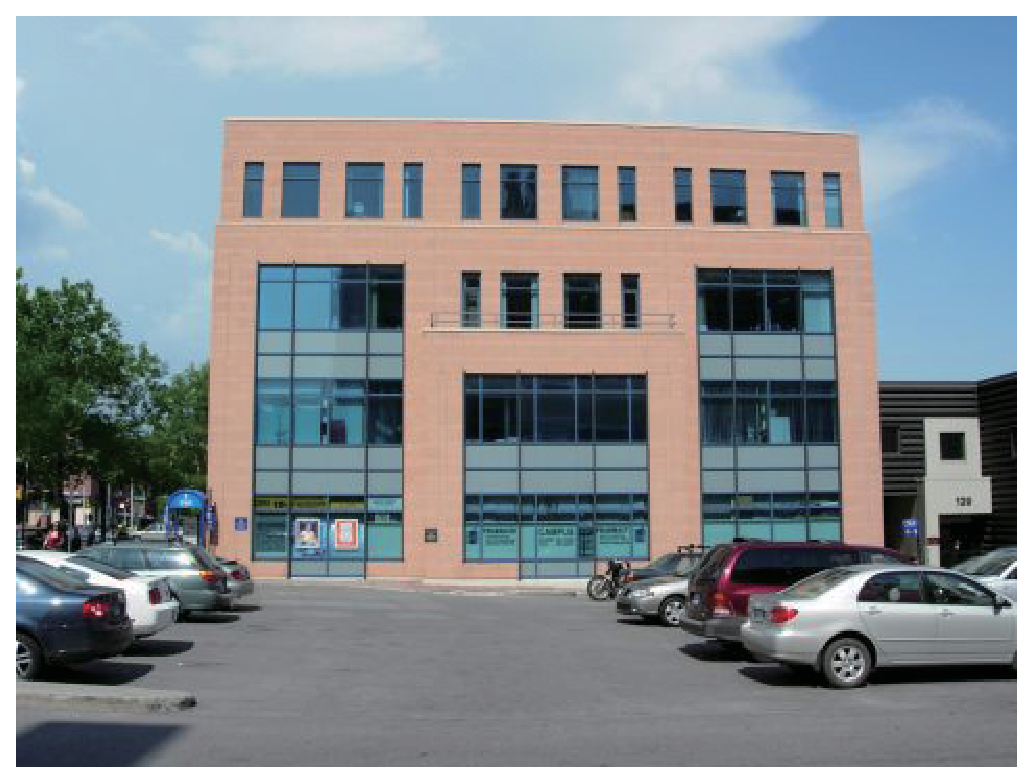
\includegraphics[width=0.4\textwidth]{figures/beforedeal}}
  \subfigure[处理后]{
            \label{fig:subfig1:subsubfig2}
            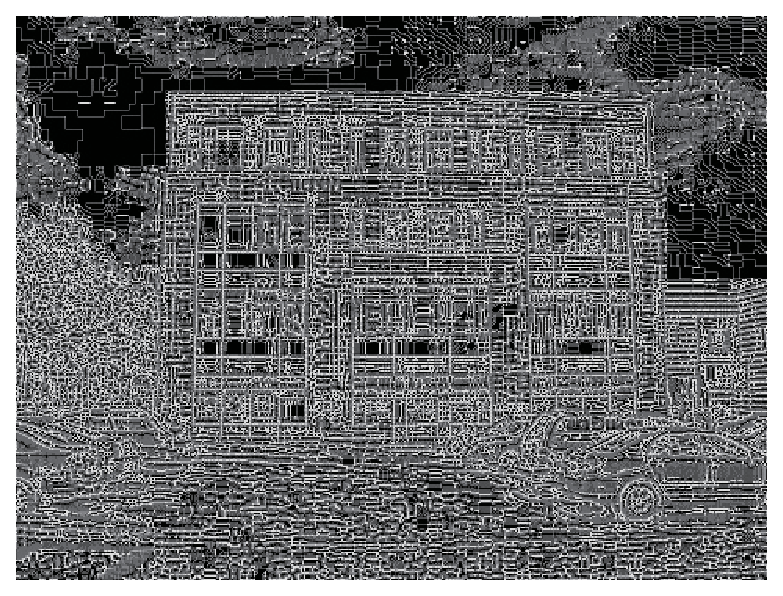
\includegraphics[width=0.4\textwidth]{figures/afterdeal}}
  \caption{处理效果}\label{fig:subfig1}
\vspace{\baselineskip}
\end{figure}
\end{verbatim}
\begin{figure}[htbp]
  \centering
  \subfigure[处理前]{
            \label{fig:subfig1:subsubfig1}
            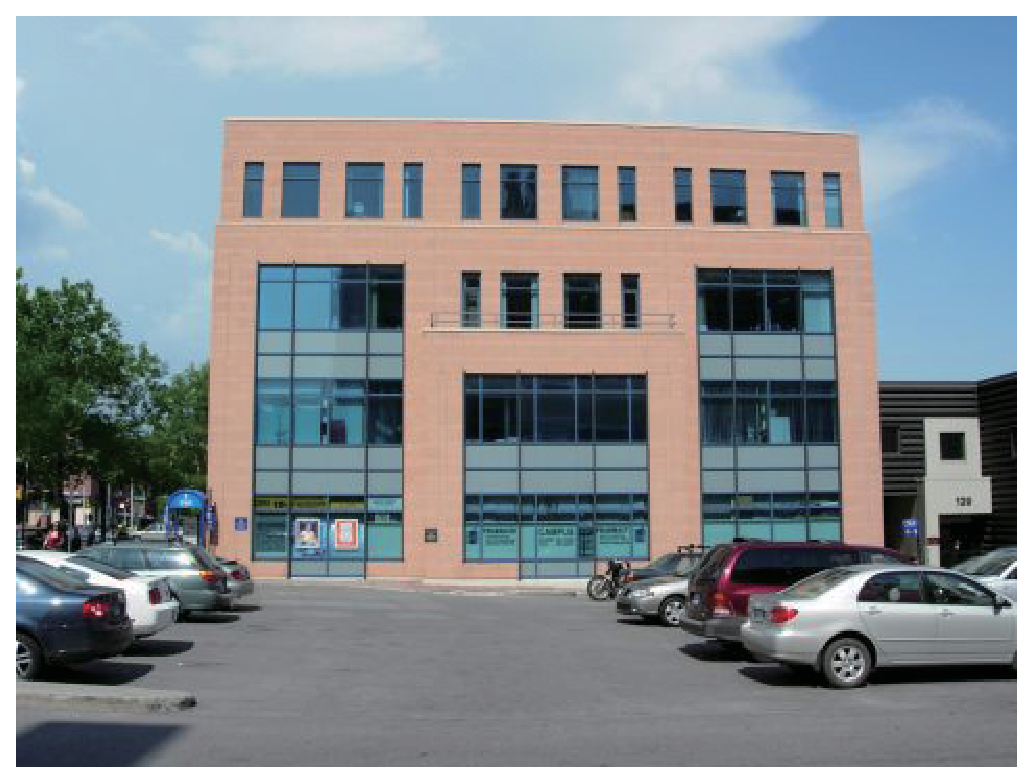
\includegraphics[width=0.4\textwidth]{figures/beforedeal}}
  \subfigure[处理后]{
            \label{fig:subfig1:subsubfig2}
            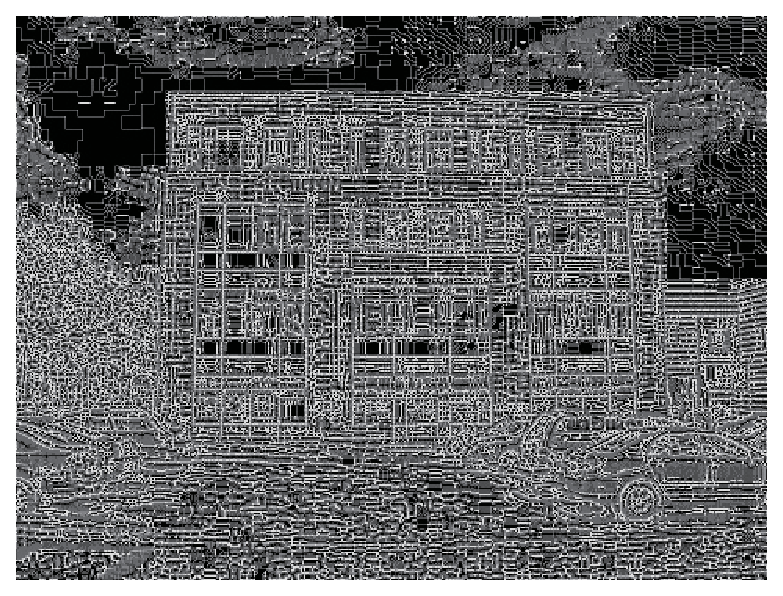
\includegraphics[width=0.4\textwidth]{figures/afterdeal}}
  \caption{处理效果}\label{fig:subfig1}
\vspace{\baselineskip}
\end{figure}
%%%%%%% 结论 %%%%%%%
% !Mode:: "TeX:UTF-8"

%%%%%%% 结论 %%%%%%%

\addcontentsline{toc}{chapter}{结\quad 论} %添加到目录中

\chapter*{结\quad 论}

山东大学(Shandong University)简称山大(SDU),是中华人民共和国教育部直属的综合性全国重点大学,是国家“211工程”、“985工程”重点建设院校。属于“111计划”、“珠峰计划”、“2011计划”  、“卓越工程师教育培养计划”、“卓越法律人才教育培养计划”、第一批“地方立法研究服务基地”高等院校,也是重点建设的高水平大学之一。


山大创建于清光绪27年(公元1901年),初名山东大学堂, 一百多年来,这所誉满海内外的百年名校历经山东大学堂、国立青岛大学、国立山东大学、山东大学等历史发展时期,迁徙分合、春华秋实,成为中国现代大学教育的重要发祥地。 学校总占地面积8000余亩(含青岛校区约3000亩), 形成了一校三地(济南、青岛、威海)八个校园的办学格局。截至2013年,学校有各类全日制学生达6万人,其中,全日制本科生41437人,研究生16034人,留学生1737人。

%%%%%%% 致谢 %%%%%%%
% !Mode:: "TeX:UTF-8"
\addcontentsline{toc}{chapter}{致\quad 谢} %添加到目录中

\chapter*{致\quad 谢}

值此论文完成之际,谨在此向多年来给予我关心和帮助的老师、同学、朋友和家人表示衷心的感谢!


同时也感谢众多的开源项目以及无数为开源而做出贡献的人们,谢谢!

......

\vspace{18pt}

谨把本文献给我最敬爱的老师!

%%%%%%%%%%  参考文献  %%%%%%%%%%
\defaultfont
\bibliographystyle{references/SDUThesis}
\phantomsection
\markboth{参考文献}{参考文献}
\addcontentsline{toc}{chapter}{参考文献}        % 参考文献加入到中文目录
\nocite{*}                                    % 若将此命令屏蔽掉,则未引用的文献不会出现在文后的参考文献中
\bibliography{references/reference}

\titleformat{\chapter}{\centering\sihao\hei}{\chaptername}{2em}{}
% !Mode:: "TeX:UTF-8"
% A4宽度 8.27 inches = 210.058 mm
% A4高度 11.69 inches = 296.926 mm
% 上左边距 > 25 mm = 0.984 inches
% 下右边距 > 20 mm = 0.787 inches
% 上边距 1.023 inches = 28 mm
% 左边距 1.3 inches = 33 mm
% 下边距 0.866 inches = 22 mm
% 右边距 0.984 inches = 25 mm
% 页眉页脚高度 1.18 inches = 29.972 mm
% 210.058 - 33 - 25 = 152.058 mm
% 296.926 - 22 - 28 = 246.926 mm
%\usepackage[a4paper,text={1\textbf{•}52.058 true mm,246.926 true mm},top= 28 true mm,left=33 true mm,head=10 true mm,headsep=6.5 true mm,foot=8 true mm]{geometry}
%\newgeometry{top= 28 true mm,bottom=22 true mm,left=13 true mm,right=25 true mm,head=10 true mm,headsep=6.5 true mm,foot=8 true mm}
%\newgeometry{text={172.058 true mm,246.926 true mm},top= 28 true mm,left=13 true mm,head=10 true mm,headsep=6.5 true mm,foot=8 true mm}
\titlecontents{chapter}[2em]{\vspace{.2\baselineskip}\bf\xiaosi\song}%
             {\prechaptername\CJKnumber{\thecontentslabel}\postchaptername\qquad}{}{}             % 设置该选项为空是为了不让目录中显示页码
\addcontentsline{toc}{chapter}{外文资料}
\setcounter{page}{1}       % 如果需要从该页开始从 1 开始编页,则取消该注释
\fancypagestyle{plain}{                              
    \fancyhf{}
    \fancyhead[L]{\song\wuhao 附录}
    \fancyhead[R]{\song\wuhao 外文资料}           
    \fancyfoot[C]{\song\xiaowu~\thepage~}
    \renewcommand{\headrulewidth}{0.5pt}
    \renewcommand{\footrulewidth}{0pt}
}
\chapter*{外文资料}
\begin{figure}[htbp] 
\centering
\vspace{-22pt}
\noindent\hspace{-1.5em}\makebox[\textwidth][l] {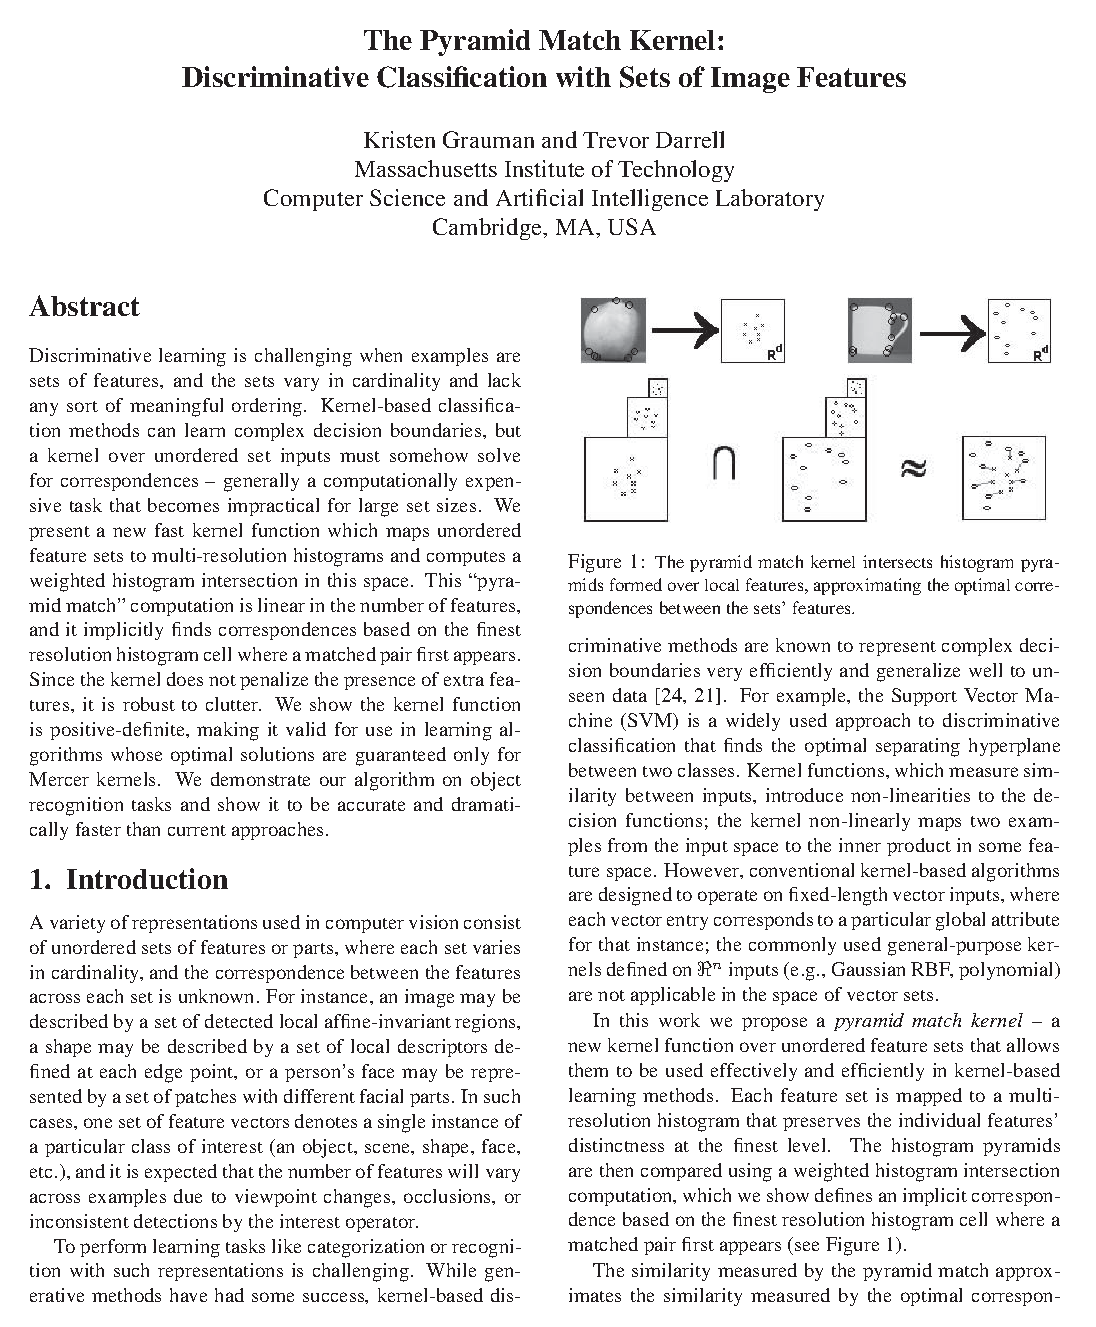
\includegraphics[width=1.08\textwidth]{figures/papers_1}}
\end{figure}
\begin{figure}[htbp] 
\centering
\noindent\hspace{-1.5em}\makebox[\textwidth][l] {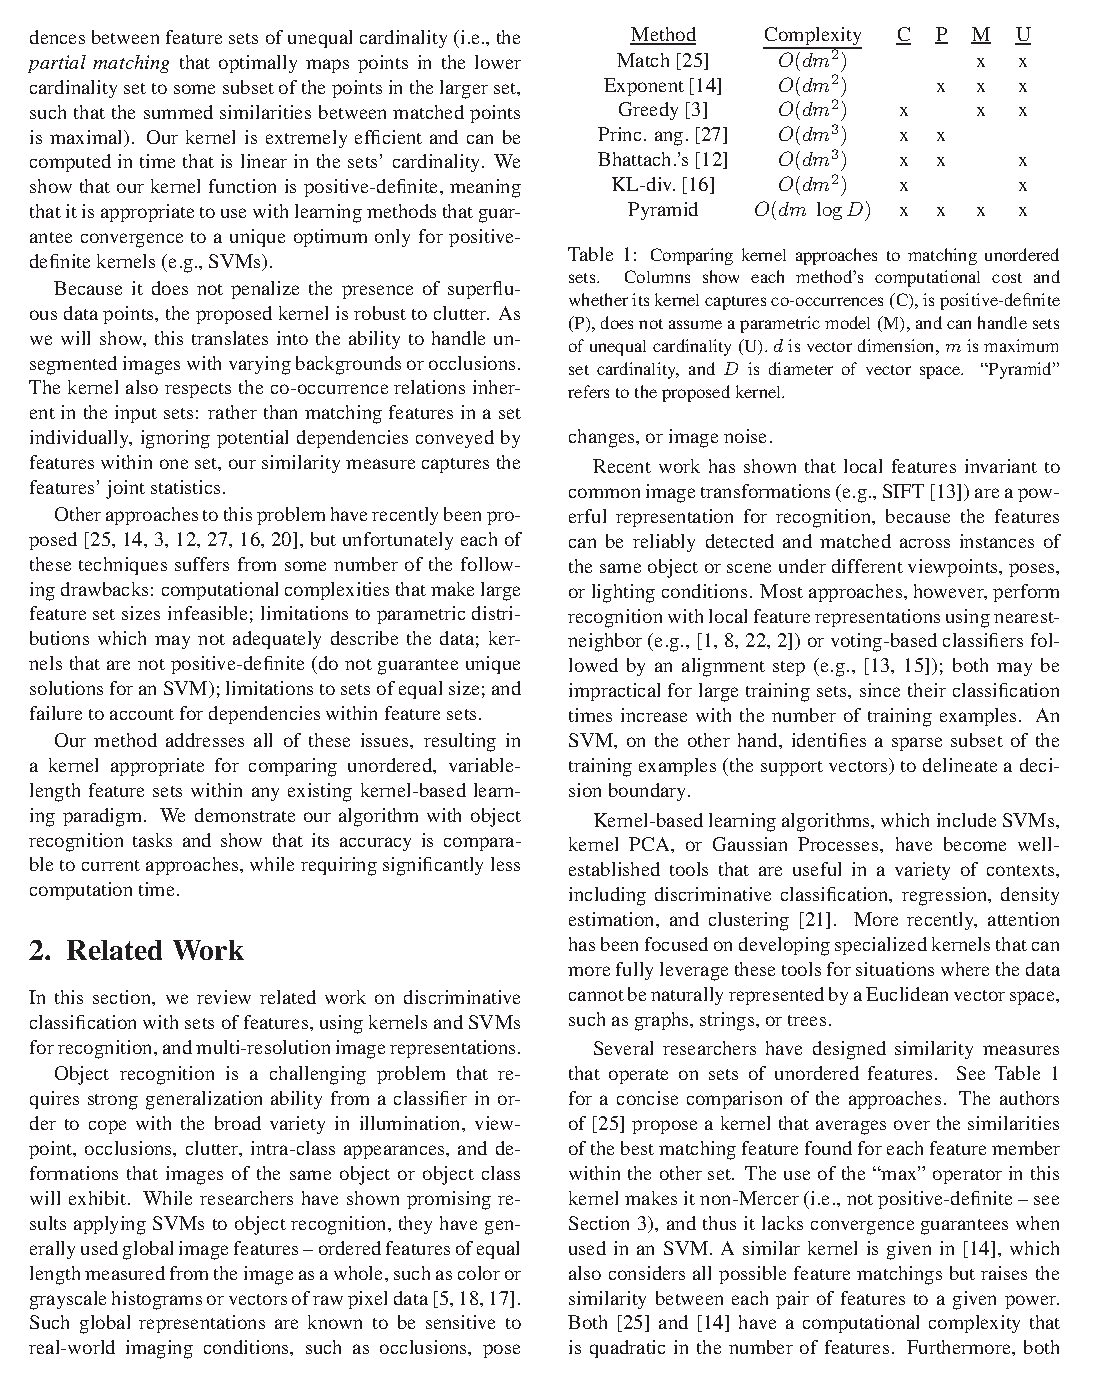
\includegraphics[width=1.08\textwidth]{figures/papers_2}}
\end{figure}

%\restoregeometry
%In this work, we propose an efficient method to automatically learn groupings over sets of unordered local features by embedding the sets into a space where they cluster according to their partial-match correspondences. Each image is decomposed into a set of local feature descriptors. Then every set is treated as a node in a graph, where an edge between two nodes (sets) is weighted according to how well some subset of the two sets features may be put into correspondence, with correspondence quality determined by descriptor similarity. A spectral clustering algorithm is then applied to the graph's affinity matrix to produce an initial set of image groupings. In an (optional) semi-supervised paradigm, we allow the user to select pairwise constraints between some number of input images, where constraints are in the form of "must-group" or "cannot-group" specifications. The affinity matrix is then modified to incorporate the user-supplied groupings prior to the spectral clustering step.
%
%
%Spectral clustering on approximate partial-match similarity scores is efficient and produces clusters that coarsely group distinct object classes. To improve specificity, and to develop a predictive classifier that can label unseen images, we develop a method to find prototypical examples in each cluster that are more likely to be class inliers, and then use these prototypes to train a predictive model.
%
%
%We detect prototype examples by examining the pattern of partial match correspondences within a cluster. Outlier cluster members are identified as those images that cause most images within the cluster to contribute an inconsistent subset of features in a partial match. With the assumption that outlier images will be less likely to match the same features as the majority of inlier images, we re-weight intracluster matching scores under a per-image mask representing the image elements that were most likely to be in correspondence when matched to other examples in the cluster.
%
%...
              % 外文资料
% !Mode:: "TeX:UTF-8"

\titlecontents{chapter}[2em]{\vspace{.5\baselineskip}\bf\xiaosi\song}
             {\prechaptername\CJKnumber{\thecontentslabel}\postchaptername\qquad}{}{}             % 设置该选项为空是为了不让目录中显示页码
\addcontentsline{toc}{chapter}{中文译文}
\setcounter{page}{1}            % 单独从 1 开始编页码
\fancypagestyle{plain}{                              
    \fancyhf{}
    \fancyhead[L]{\song\wuhao 附录}            
    \fancyhead[R]{\song\wuhao 中文译文}           
    \fancyfoot[C]{\song\xiaowu~\thepage~}
    \renewcommand{\headrulewidth}{0.5pt}
    \renewcommand{\footrulewidth}{0pt}
}
\chapter*{中文译文}

本文\footnote{基于双空间金字塔匹配核的图像目标分类.陈海林,吴秀清} 提出一种基于局部特征的双空间金字塔匹配核(bi-space pyramid match kernel,BSPM)用于图像目标分类。利用局部特征在特征空间和图像空间建立统一的多分辨率框架,以便较好地表达图像的语义内容。该方法同时在特征空间和图像空间建立金字塔型结构,通过适当匹配可以得到正定核函数,该函数具有线性计算复杂度,可以运用于基于核的学习算法。将BSPM嵌入支持向量机对公共数据库中图像目标进行分类,实验结果表明该方法对图像具有良好的分类能力,优于词汇导向的金字塔匹配核和空间金字塔匹配核.


图像目标的分类、识别是计算机视觉和模式识别领域的一个重要研究问题。由于图像目标存在视角变化、亮度变化、尺度、目标变形、遮挡、复杂背景以及目标类内差别等影响,使得图像目标的分类识别非常困难。针对这些问题,已提出具有各种不变性的局部特征[1-2],如SIFT(scale invariant featuret ransform)[3]。Fergus等[4]提出基于局部特征的生成模型用于图像分类,Berg等[5]和Lazebnik等[6]提出基于几何对应的图像分类方法,这些方法没能较好地利用局部特征在特征空间的结构特性,而且计算复杂度很高[7]。最近提出基于特征包(bags-offeatures)的方法对图像目标分类[1,8-11],取得了良好的效果,但这些方法没有利用局部特征之间的空间关系。Grauman提出的金字塔匹配核(pyramid match kernel,PMK)[9]具有比较优越的匹配、分类性能,但不适用于高维特征。最近,Grauman提出词汇导向的金字塔匹配核(vocabulary-guided pyramid match kernel,VGPM)[10],并取得良好的性能,该方法首先利用一系列局部特征在特征空间建立金字塔型结构,然后将图像的局部特征嵌入金字塔结构,形成特征空间多分辨率直方图,再计算直方图匹配,得到核函数。为了利用局部特征在图像空间的位置关系,Lazebnik等[7]借鉴Grauman[9]的金字塔匹配核的思想,提出空间金字塔匹配核(spatial pyramidmatching kernel,SPM),首先对局部特征量化,在二维图像空间建立金字塔,然后计算加权的子图像区域局部特征直方图交叉。

...
              % 中文译文
% !Mode:: "TeX:UTF-8"

\titlecontents{chapter}[2em]{\vspace{.5\baselineskip}\bf\xiaosi\song}
             {\prechaptername\CJKnumber{\thecontentslabel}\postchaptername\qquad}{}{}             							% 设置该选项为空是为了不让目录中显示页码
\addcontentsline{toc}{chapter}{源代码}
\setcounter{page}{1}    	% 单独从 1 开始编页码
\fancypagestyle{plain}{                              
    \fancyhf{}
    \fancyhead[L]{\song\wuhao 附录}            
    \fancyhead[R]{\song\wuhao 源代码}           
    \fancyfoot[C]{\song\xiaowu~\thepage~}
    \renewcommand{\headrulewidth}{0.5pt}
    \renewcommand{\footrulewidth}{0pt}
}

\chapter*{源代码}
\noindent
file:main.c
\begin{lstlisting}
int main(int argc, char ** argv) {
    printf("Hello world!\n");
    return 0;	/*`程序运行完毕`*/
}
\end{lstlisting}

...
              	   % 源代码
\clearpage
\end{document}                                 % 结束全文
